\section{Reinforcement Learning (RL)}~\label{ssec:rl}
Please note that this is an aggressively shortened summary. For a deeper introduction please refer to \cite{SB_all}.
The Reinforcement Learning problem originates from the idea of learning by interacting with an environment. The object that is learning is doing so by retrieving information from cause and effect. The causal model that is learned in such a way is updated with each change of the environment that can be related to some action. Therefore, the learned model fits the true model increasingly better with the number of induced causes and observed effects.\\
This type of learning problem can be modeled by "Finite Markov Decision Processes". Such processes usually need the following elements:\\

\begin{itemize}
	\item \textbf{Environment} The environment is a dynamic model of some complex process.
	\item \textbf{State} The state $s_t$ is generated by the environment. It changes over time according to the dynamics within the environment.
	\item \textbf{Action} An action $a_t$ is a cause that might change the state of the environment. Actions are produced by the agent.
	\item \textbf{Reward} The reward $r_t$ is a scalar value that is produced by the environment and received by the agent.
	\item \textbf{Agent} The agent is a instance which generates actions and observes the caused change of the state of the environment.
	\item \textbf{Policy} A policy $\pi(a_t|s_t)$ is a probability distribution over the set of possible actions at a time step. A agent is essentially defined by its policy as each action that is taken is sampled from that policy.
\end{itemize}

The model with its signal flows is depicted in figure \ref{fig_rl_gen}

\begin{figure}
	\centering
	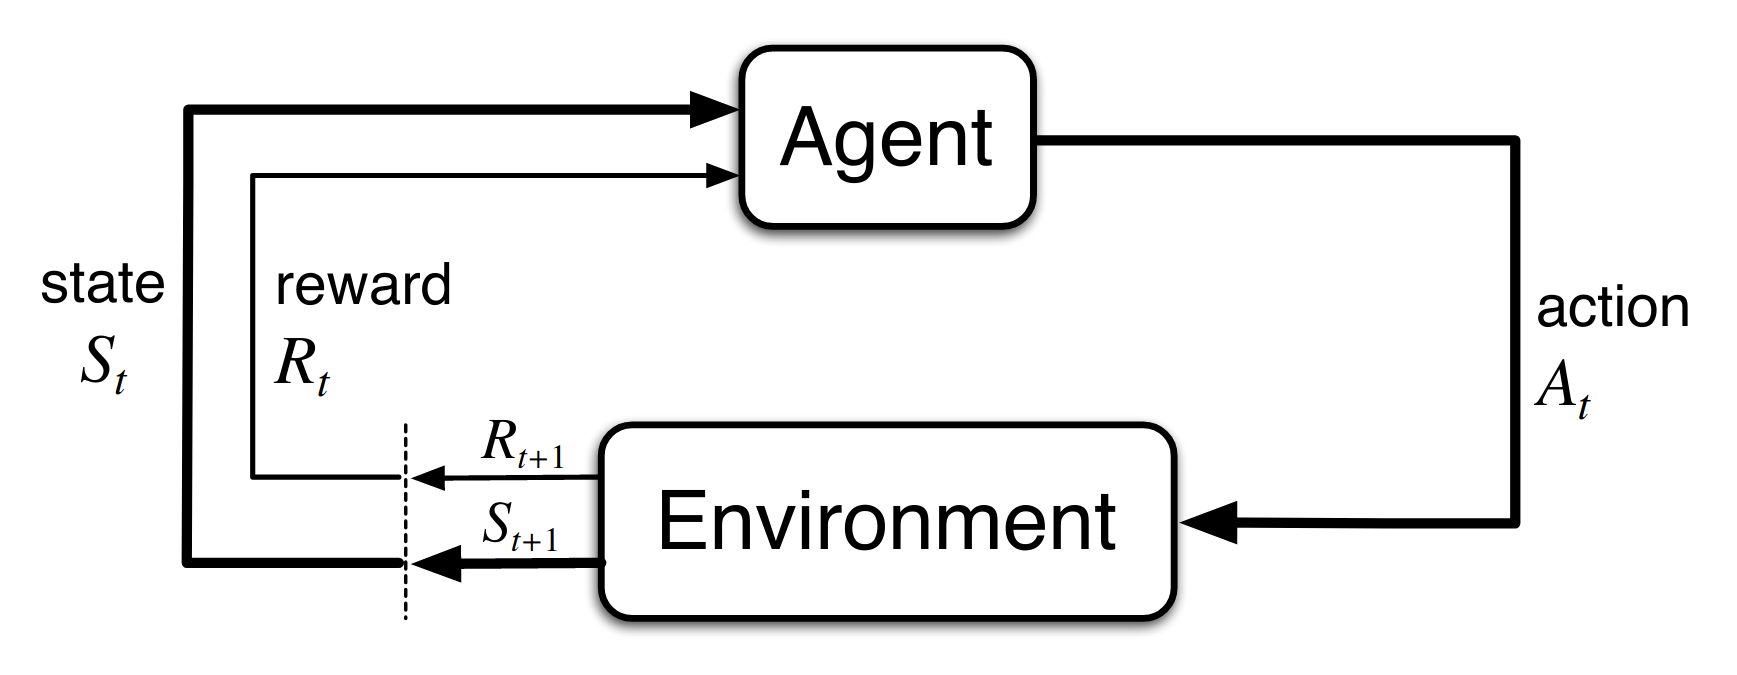
\includegraphics[width=0.8\textwidth]{figures/rl/agent_env_interface}
	\caption{agent environment interaction \cite{SB_all}}
	\label{fig_rl_gen}
\end{figure}

All signals in this model are time dependent. 
Such a model satisfies the Markov Property if next $s'$ and reward $r$ only depend on the current action-state tuple $(s, a)$. If assuming finite state and action spaces together with the Markov Property gives a Finite Markov Decision Process. The environment dynamics can therefore be represented by the bivariate probability distribution
\begin{align}
	p(s', r|s, a) = Pr\{r_{t+1}=r, s_{t+1} = s' | s_t=s, a_t=a\}
\end{align}
Further, if $a_t$ is sampled from $\pi(a_t|s_t)$ the Markov Property induces conditional independence of $(s_{t-1}, r_{t-1})$ and $(s_{t+1}, r_{t+1})$ given $s_t$. \\

The agents task is to predict a policy that maximizes the expected future rewards. This objective is given by
\begin{align}
	\argmax_{\pi}\mathop{\mathbb{E}}_{p_{\pi}}\left[\sum_{t=0}^T r_t | s_0\right]
\end{align}
Here T marks the time limit of the process and $p_{\pi}$ represents the environment dynamics following a action history sampled from $\pi$.\\

\subsection{Value functions}
Most methods of solving eq. (1.2) use so estimations of so called value functions. This are functions that provide a quality measure for an agent evaluating a state-action tuple. \\
Commonly three value functions are used. The state-value function, the action-value function and the advantage-value function. They all depend on the expected discounted future rewards
\begin{align}
	g_t = \sum^{T-t-1}_{k=0} \gamma^k r_{t+k+1} .
\end{align}
Here $\gamma$ is referred to as the discount factor. Its value usually determines how prospective future rewards are weighted in the value function. E.g if $\gamma<1$ rewards that are closer to $t$ get a higher weight than those that are occuring at a later time. For $\gamma>1$ the contrary holds.\\
The state-value function is defined by
\begin{align}
	V_{\pi}(s) = \mathop{\mathbb{E}}_{p_{\pi}}\left[g_t|s_t=s \right]\text{,}
\end{align}
the action-value by
\begin{align}
	Q_{\pi}(s, a) = \mathop{\mathbb{E}}_{p_{\pi}}\left[g_t|s_t=s, a_t=a \right]
\end{align}
and finally the advantage-value by
\begin{align}
	A_{\pi}(s, a) = Q_{\pi}(s, a) - V_{\pi}(s)
\end{align}
it follows
\begin{align}
	V_{\pi}(s) = \mathop{\mathbb{E}}_{a\sim\pi}\left[ Q_{\pi}(s, a)\right]
\end{align}

\noindent Usually the objective is to maximize either one or both of the value functions.
Note that, $\max_{\pi}V_{\pi}(s)$ and $\max_{\pi}Q_{\pi}(s, a)$ satisfy Bellman's principle of optimality. Hence they can be solved exactly by Dynamic Programming. This is referred to as the tabular solution. However for most problems this is not feasible and the value functions are approximated by neural networks. \\

\subsection{Q-learning}
Q-learning is a method to find the action-value maximizing policy by using temporal differences. This often the backbone of policy gradient algorithms. Let
\begin{align}
\pi(\cdot|s) = \softmax_{a}Q_{\pi}(s, a)
\end{align}
then the objective is to approximate $Q_{\pi}$ which is achieved by the temporal difference loss
\begin{align}
\mathcal{L}_{TD} = \frac{1}{2} \left(r_{t+1} + \gamma \max_{a}Q_{\pi}(s_{t+1}, a) - Q_{\pi}(s_t, a_t)\right)^2
\end{align}
this kind of approximation is usually referred to as one step TD method. The optimality follows directly and the convergence of the approximation under certain conditions has been proven in \cite{SBQL}.\\
In contrast to one step TD methods there are Monte Carlo methods which collect the loss over whole episodes where one episode is defined by the history of temporal differences between a starting state and an end state. This methods are often solved by eligibility traces \cite{SBeligibility}. \\
Optimizing eq (1.8) is referred to as on-policy policy optimization where the target policy $\pi$ is the policy which is used when actions are sampled. This however is problematic as the target policy is defined by eq (1.7) depending on $q_{\pi}$ which is not trustworthy as this is the function that is to be approximated. In order to have more control over the sampling of actions which is usually referred to as exploration a data collection policy $\mu(a|s)$ is used. Therefore in an off-policy setting eq (1.8) becomes
\begin{align}
\mathcal{L}_{TD} = \frac{1}{2} \left(r_{t+1} + \gamma \max_{a}Q_{\mu}(s_{t+1}, a) - Q_{\mu}(s_t, a_t)\right)^2\text{.}
\end{align}
and during inference 
\begin{align}
\bar{\pi}(\cdot|s) = \softmax_{a}Q_{\mu}(s, a)
\end{align}
is used. There are many solutions to overcome the distribution mismatch between $\pi$ and $\mu$. Many use importance sampling or variance reduction techniques.\cite{liu2018breaking}

\subsection{Policy gradient methods}

This class of methods optimizes the parameters $\theta$ that define the statistics of a policy $\pi_\theta(a|s)$. Let 
\begin{align}
\rho(\pi) = \sum_{t=1}^{\infty}\mathop{\mathbb{E}}_{\substack{s\sim d_\pi(s) \\ a\sim \pi(a|s)}} \left[ r_t|s_0 \right]
\end{align}
be the expected, discounted future reward per step and let
\begin{align}
d_\pi(s) = \sum_{t=0}^\infty \gamma^t Pr\left\{s_t=s|s_0, \pi\right\}
\end{align}
be the discounted stationary distribution of states under $\pi$. Then
\begin{align}
\frac{\partial\rho_\pi}{\partial\theta} = \sum_s d_\pi(s)\sum_a \frac{\partial\pi(a|s)}{\partial\theta} \bar{Q}_\pi(s,a)
\end{align}
Is the policy gradient with which gradient ascent on the policy can be performed in order to maximize $\rho$. A proof and a thorough discussion can be found in \cite{PGBS}. Note that the policy gradient is on-policy and that $\bar{Q}_\pi$ is an approximation of $Q_\pi$.\\
Since $\pi$ is a probability distribution it follows $\sum_a\frac{\partial\pi(a|s)}{\partial\theta}=0, \forall s \in S$. Therefore
\begin{align}
\frac{\partial\rho_\pi}{\partial\theta} = \sum_s d_\pi(s)\sum_a \frac{\partial\pi(a|s)}{\partial\theta}\left[ \bar{Q}_\pi(s,a)+b(s)\right],\text{\hspace{12mm}} b:S\rightarrow \mathop{\mathbb{R}}
\end{align}
the function $b$ is called a baseline and is often used to reduce variance and bias of the gradient ascent update step. Using $\frac{\nabla_\theta\pi(a|s)}{\pi(a|s)} = \nabla_\theta ln(\pi(a|s))$ and $\mathop{\mathbb{E}}_{x\sim p(x)}[f(x)] = \sum_{x}p(x)f(x)$, rewriting eq (1.13) yields
\begin{align}
\frac{\partial\rho_\pi}{\partial\theta} = \mathop{\mathbb{E}}_{\substack{s\sim d_\pi(s) \\ a\sim \pi(a|s)}}\left[ \nabla_\theta ln (\pi(a|s))\left[ \bar{Q}_\pi(s,a)+b(s)\right]\right]
\end{align}
In practice where there are large state and action spaces the expectations w.r.t $s$ and $a$ become infeasible to obtain. Using $\mathop{\mathbb{E}}_{x\sim p(x)}[f(x)] = \frac{1}{n}\sum_{n}f(x), n\rightarrow\infty, x\sim p(x)$ , ample based learning uses enough samples of $s$ and $a$ in order to obtain a good enough approximation of the expectations. Therefore eq. (1.15) becomes

\begin{align}
\frac{\partial\rho_\pi}{\partial\theta} = \frac{1}{n}\sum_{n} \nabla_\theta ln (\pi(a|s))\left( \bar{Q}_\pi(s,a)+b(s)\right),\text{\hspace{8mm}} s\sim d_\pi(s), \text{\hspace{4mm}} a\sim \pi(a|s), \text{\hspace{4mm}} n\rightarrow\infty
\end{align}

This leads to Actor Critic methods (A2C) where there are two instances that are updated in a turn based fashion. The critic is the value-function approximation and the actor is approximating the policy. Intuitively the critic evaluates the action taken by the actor who uses this evaluation to scale its gradient update (this is the role of $\bar{q}_\pi$ in eq (1.13)).

\subsection{Maximum Entropy Reinforcement Learning}
In off-policy settings it is common to use a data collection policy $\mu$ which has a large entropy in order to encourage exploration of the action and state spaces. The principle of maximum causal entropy has been introduced by \cite{AAAIziebert} and has been elaborated on among others by \cite{DBLP:journals/corr/HaarnojaTAL17}. The key idea is to incorporate an entropy term into the objective function acting like a regularizer. 

\begin{align}
\rho^{\mathcal{H}}(\pi) = \sum_{t=1}^{\infty}\mathop{\mathbb{E}}_{\substack{s_t \sim d_\pi(s_t) \\ a_t \sim \pi(a_t|s_t)}} \left[ r_t + \alpha(t) \mathcal{H}(\pi(\cdot | s_t))|s_0 \right]
\end{align}
Here $\alpha$ is a non-negative regularization weight which is usually monotonically decreasing with increasing $t$ and $\mathcal{H}$ is some entropy measure. If $\alpha$ becomes $0$ eq. (1.17) becomes equal to eq. (1.11), therefore, intuitively $\alpha$ should be high in the early phase of training the policy and the value function and converge to $0$ as the policy gets closer to the perfect policy and therefore can afford to have more certainty in its prediction.
This objective is on-policy and still gives control over the exploration behavior. Usually it does not bother if the policy has high entropy, since during inference the action where "\pi" has maximum probability is selected. This makes especially unimodal distributions attractive. They fixate on single actions and they imply few parameters only that need to be learned (e.g. mean and variance of normal distributions). However often more expressive multimodal distributions fit the true distribution which is approximated better. 
In \cite{DBLP:journals/corr/abs-1906-02771} this idea has been extended by using  normalizing flows. Normalizing flows \cite{papamakarios2019normalizing} are based on the idea of transforming a probability density function by letting each sample undergo a transformation. If this transformation is a diffeomorphism the probability of the transformed sample can be determined. Let $T$ be a diffeomorphism of a real vector $u$ sampled from $p_u(u)$.

\begin{align}
	x=T(u) \text{\hspace{5mm}where\hspace{5mm}} u\sim p_u(u)
\end{align}
then
\begin{align}
p_x(x)=p_u(T^{-1}(u)) |detJ_T(u)|^{-1}
\end{align}
where $J_T(u)$ is the Jacobian matrix of $T$ w.r.t. $u$. I practice an invertible neural network can be trained to transform a simplistic density function into a more expressive one.\\
E.g. let the agent predict mean and variance of a Normal distribution. Actions are the in the data collection process sampled from a transformed Normal distribution where the transform encourages entropy and maybe also multiple modes. Assuming the sampling happened using reparametrization the log probabilities and their gradient in eq (1.14) can still be calculated. This is a on-policy training with a expressive density function and the advantage is that easy reparameterization tricks can still be used since the sampling itself is happening from the base distribution.

\subsection{Soft Actor-Critic (SAC)}\label{ssec:sac}
This algorithm was introduced by \cite{haarnoja2018soft}. They aim to maximize the objective in eq. (1.17). Particularly they focus on the selection of the weight factor $\alpha$ and show, that it can be seen as a learnable parameter which is trained jointly with actor and critic networks.\\
SAC is derived from the soft policy iteration where the temporal difference equation for the action value depends on the soft value function which is
\begin{align}
	V_{\pi}(s_t) = \mathop{\mathbb{E}}_{a \sim \pi(a|s_t)} \left[ Q_{\pi}(s_t, a) - \alpha log( \pi(a|s_t)) \right]
\end{align}
the negative log probabilities are the entropy measure in eq. (1.18). The action value function loss yields
\begin{align}
	\mathcal{L}_{critic} = \frac{1}{2}(Q_{\pi}(s_t, a_t) - (\gamma \mathop{\mathbb{E}}_{s_{t+1} \sim d_{\pi}(s)} \left[ V_{\pi}(s_{t+1})\right] + r_t)) ^ 2
\end{align}

For the policy improvement step the policy is updated such that it approximates $\softmax_a(\frac{1}{\alpha}Q_{\pi}(s, a))$ where $Q_{\pi}$ is the soft action value function, learned by minimizing eq (1.21). The loss for the policy then yields

\begin{align}
\mathcal{L}_{actor} = DKL_{a}\left[ \pi(a| s_t) \bigg|\bigg| \frac{exp(\frac{1}{\alpha} Q_{\pi}(s_t, a))}{Z(s_t)} \right]
\end{align}

here, $DKL_{a}$ is the Kullback Leibler Divergence over the actions. $Z(s_t)$ is the partition function of the distribution. 

\begin{align}
	Z(s_t) = \sum_a Q_{\pi} (s_t, a)
\end{align}

It is usually too expensive to evaluate $Z(s_t)$ since it involves integrating/summing over the action value space which means many forward passes through the neural network that represents $Q_{\pi}$. Since $\mathcal{L}_{actor}$ is minimized by gradient descent methods only the gradient is needed. If one expands the KL-divergence term, $Z(s_t)$ becomes additive and therefore vanishes once the gradient is obtained.\\
Note that $\alpha$ gives control over the differences between action values and therefore over the entropy of the resulting distributution. \emph{lemma 2} in \cite{haarnoja2018soft} claims the improvement of $Q_{\pi}$ with each optimization step of $\mathcal{L}_{actor}$.\\
The gradient of eq. (1.23) w.r.t. the parameters $\theta$ of $\pi$ yields

\begin{align}
\nabla_\theta \mathcal{L}_{actor} = \nabla_\theta \mathop{\mathbb{E}}_{\substack{s_t \sim d_\pi(s_t) \\ a_t \sim \pi(a_t|s_t)}} \left[ \alpha log(\pi(a_t|s_t)) - Q_\pi(s_t, a_t) \right]
\end{align}

approximating eq. (1.24) by a sample based method yields

\begin{align}
\nabla_\theta \bar{\mathcal{L}}_{actor} = \nabla_\theta \left[ \alpha log(\pi(a_t|s_t)) - Q_\pi(s_t, a_t) \right]
\end{align}

minimizing this loss by a gradient descent method involves backpropping through a sampling procedure. This can be made differentiable by the reparameterization trick \cite{kingma2013autoencoding}.

\cite{haarnoja2018soft} also provides a method to determine the entropy adjustment $\alpha$ such that it takes the minimal value needed to maximize the maximum entropy objective eq. (1.17) assuming a fixed policy $\pi$.

In practice, reinforcement learning problems have high dimensional action spaces but only one dimensional rewards. Therefore the learned action value function of the critic is also one dimensional in contrast to the actor who predicts the statistics of the policiy for each action dimension. Then the joint probability is the product of probabilities over all actions. This results in summing the log probabilities in eq. (1.25)

\subsection{Common optimization methods}\label{ssec:common_opt}
There are numerous optimization methods for reinforcement learning problems. This is just a listing of only very few but important ones, reviewed and tested in \cite{hessel2017rainbow}.

\begin{itemize}
	\item \textbf{Double Q-learning} \label{text:doublQ} \cite{DBLP:journals/corr/HasseltGS15} Conventional Q-learning is affected by an overestimation bias of action values. Decoupling the action selection from its evaluation by learning two action value networks independently resulting in the loss
	
	\begin{align}
		\mathcal{L}_{TD} = \frac{1}{2} \left(r_{t+1} + \gamma Q_{\pi}^{(\bar{\phi})} \left( s_{t+1}, \argmax_{a}Q_{\pi}^{(\phi)}(s_{t+1}, a) \right) - Q_{\pi}^{(\phi)}(s_t, a_t)\right)^2\text{.}
	\end{align}
	Here $\phi$ and $\bar{\phi}$ are the parameters of the independently trained action value functions respectively. A similar method trains two action value functions independently and and takes for all evaluations the min value of the two network predictions. Both methods show a reduction in overestimation as shown in \cite{DBLP:journals/corr/HasseltGS15}.
	
	\item \textbf{Prioritized replay} During data collection, the tuples $(s_t, a_t, r_{t+1}, s_{t+1})$ are stored in a replay buffer and during training phases then sampled uniformly from the buffer. In \cite{schaul2015prioritized} the sampling is not uniform but rather with a probability $p_t$ relative to the last encountered loss of that replay tuple.
	\begin{align}
		p_t \propto \mathcal{L}_{TD} ^ \omega \text{.}
	\end{align}
	Raising the loss to the power of the parameter $\omega$ determines the shape of the distribution. New transitions that did not produce a loss yet are always sampled with maximum priority.
	
	\item \textbf{Multi-step learning} Q-learning bootstraps from single step temporal difference losses. \cite{SBQL} introduced multi-step temporal differences which is the transition from Monte Carlo methods to single step temporal difference methods. The $n$-step return is defined as 
	
	\begin{align}
		r_t^{(n)} \equiv \sum_{k=0}^{n-1} \gamma_t^{k} r_{t+k+1}
	\end{align}
	
	then the multi step TD loss yields,
	
	\begin{align}
		\mathcal{L}_{TD} = \frac{1}{2} \left(r_{t+1}^{(n)} + \gamma^{n} \max_{a}Q_{\pi}(s_{t+n}, a) - Q_{\pi}(s_t, a_t)\right)^2
	\end{align}
	
	optimizing multistep TD losses with $n$ sampled uniformly from the interval $[1..T]$ results in faster learning as shown in \cite{SBQL}.
	
	\item \textbf{Dueling networks} This is an optimization method based on the neural network atrchitecture of value functions in value based RL and was introduced by \cite{DBLP:journals/corr/WangFL15}. It features one state-value and one advantage-value stream of computation that both share a common state feature extractor network $f(s)$. This leads to this factorization of action-values
	\begin{align}
		Q_{\pi}^{(\phi)}(s, a) = V_{\pi}^{(\eta)}(f^{(\xi)}(s)) + A_{\pi}^{(\psi)}(f^{(\xi)}(s), a) - \frac{\sum_{a'} A_{\pi}^{(\psi)}(f^{(\xi)}(s), a')}{N_{actions}}
	\end{align}
	
	Here $\eta, \psi$ and $\xi$ are the parameters of the state-value function, the advantage-value function and the state feature extractor respectively. $\phi$ is the concatenation of $\eta, \psi$ and $\xi$.\\
	The last term in eq. (1.31) approximates $\mathop{\mathbb{E}}_{a' \sim \pi} A_{\pi}^{(\psi)}(f^{(\xi)}(s), a')=0$, this equality follows from combining eq (1.6) and eq(1.7). Then eq. (1.31) follows from eq (1.4), eq (1.5) and eq (1.6).\\
	This method outperforms vanilla, value based RL methods on common RL benchmarks. 
	
\end{itemize}

\subsection{Reparameterization} \label{ssec:reparam}

\subsection{Normalizing flows}\label{ssec:norm_flows}
